\documentclass{beamer}

\usepackage{helvet}
\usepackage{hyperref, graphicx}
\usepackage{amsthm}
\usepackage{etoolbox}
%\usepackage{multicol}
\usepackage{tikz}
\usepackage{ulem}

\usetheme{default}
\setbeamertemplate{navigation symbols}{}
\AtBeginSection[ ]
{
\begin{frame}{Outline}
    \tableofcontents[currentsection]
\end{frame}
}

% Default fixed font does not support bold face
\DeclareFixedFont{\ttb}{T1}{txtt}{bx}{n}{11} % for bold
\DeclareFixedFont{\ttm}{T1}{txtt}{m}{n}{12}  % for normal - use in headings

% Custom colors
\usepackage{color}
\definecolor{TUGray}{RGB}{101,101,137}
\definecolor{TUBlack}{RGB}{30,0,0}
\definecolor{mygreen}{RGB}{45,111,63}
\definecolor{keywords}{RGB}{205,114,0}
\definecolor{comments}{RGB}{181,51,139}
\definecolor{strings}{RGB}{58,144,81}
\definecolor{numeric}{RGB}{66,110,176}
\definecolor{linos}{rgb}{0.4,0.4,0.4}
\definecolor{links}{rgb}{0,0.4,0.75}

\definecolor{bggray}{RGB}{232, 233, 235}

\usecolortheme[named=mygreen]{structure}
\setbeamercolor{normal text}{fg=TUBlack}\usebeamercolor*{normal text}

\setbeamercolor{codecol}{fg=TUGray!25!black,bg=bggray}

\hypersetup{colorlinks, linkcolor=links, urlcolor=links}

\usepackage[T1]{fontenc}
\usepackage[sfdefault,scaled=.85]{FiraSans}
\usepackage{newtxsf}

\usepackage{listings}

\newtoggle{InString}{}% Keep track of if we are within a string
\togglefalse{InString}% Assume not initally in string

\newcommand\digitstyle{\color{numeric}}
\makeatletter
\newcommand{\ProcessDigit}[1]
{%
  \ifnum\lst@mode=\lst@Pmode\relax%
   {\digitstyle #1}%
  \else
    #1%
  \fi
}
\makeatother

\lstset{literate=%
    {0}{{{\ProcessDigit{0}}}}1
    {1}{{{\ProcessDigit{1}}}}1
    {2}{{{\ProcessDigit{2}}}}1
    {3}{{{\ProcessDigit{3}}}}1
    {4}{{{\ProcessDigit{4}}}}1
    {5}{{{\ProcessDigit{5}}}}1
    {6}{{{\ProcessDigit{6}}}}1
    {7}{{{\ProcessDigit{7}}}}1
    {8}{{{\ProcessDigit{8}}}}1
    {9}{{{\ProcessDigit{9}}}}1
	{<=}{{\(\leq\)}}1
	{>=}{{\(\geq\)}}1,
	% morestring=[b]",
    % morestring=[b]',
    % morecomment=[l]{//},
}

\lstdefinelanguage{Pseudo}{
    morekeywords={return, while, if, for, input},
    morecomment=[l]{\#},
}

% Pseudocode style
\newcommand\pseudostyle{\lstset{
language=Pseudo,
basicstyle=\fontfamily{ccr}\scriptsize,
commentstyle=\it\scriptsize\color{linos},
keywordstyle=\it\bfseries\scriptsize,
mathescape=true,
literate=
    {=}{$\leftarrow{}$}{1}
    {==}{$={}$}{1}
    {<=}{{\(\leq\)}}1
	{>=}{{\(\geq\)}}1,
xleftmargin=18pt,
xrightmargin=4pt,
aboveskip=12pt,
belowskip=0pt,
frame=tB,
keepspaces=true
}}

% Python style for highlighting
\newcommand\pythonstyle{\lstset{
language=Python,
basicstyle=\ttfamily\tiny,
numbers=left,
numberstyle=\tiny\color{linos},
morekeywords={self, np},              % Add keywords here
keywordstyle=\tiny\color{keywords},
commentstyle=\it\tiny\color{comments},    % Custom highlighting style
stringstyle=\tiny\color{strings},
xleftmargin=18pt,
xrightmargin=4pt,
aboveskip=0pt,
belowskip=0pt,
escapeinside={(*@}{@*)},
frame=l,                         % Any extra options here
showstringspaces=false,
keepspaces=true
}}

% Pseudocode environment
\lstnewenvironment{pseudo}[1][]
{
    \pseudostyle
    \lstset{
        #1
    }
}
{}

% Python environment 
\lstnewenvironment{python}[1][]
{
	\pythonstyle
	\lstset{
	#1
	}
}
{}

% wrap the Python environment
\newenvironment{codeblock}
    {\hfill\begin{beamerboxesrounded}[lower=codecol, width=0.8\textwidth]
    \medskip

    }
    { 
    \end{beamerboxesrounded}\hfill
    }

\theoremstyle{example}
\newtheorem{question}{Question}

\newcommand{\ct}[1]{\lstinline[language=Python]!#1!}
\newcommand{\ttt}[1]{{\small\texttt{#1}}}
\newcommand{\lsitem}[2]{\ttt{{#1}[}\ct{#2}\ttt{]}}

\author{Chris Cornwell}
\date{Feb 27, 2025}
\title{Logistic Regression}

\begin{document}

\begin{frame}
\titlepage
\end{frame}

\begin{frame}
\frametitle{Outline}
\tableofcontents
\end{frame}

\section{Reconsidering the Half-space Model}

%%%%
\begin{frame}
\frametitle{Decision boundaries}
For model $h$, made for classification task (with data points ${\bf x}\in\mathbb R^d$), write $C_y\subset \mathbb R^d$ for the set of points with label $y$, i.e.,
    \[C_y = h^{-1}(y) = \{{\bf x}\in\mathbb R^d\ |\ h({\bf x}) = y\}.\]

\pause
Say $y \ne y'$ and a point is in the boundary of both $C_y$ and $C_{y'}$. We say that point is on a \textbf{decision boundary} of the model. In a half-space model (last lecture), the hyperplane determined by ${\bf w}$ and $b$ is the decision boundary.

\pause
The Perceptron algorithm might produce a model with many data points that are \emph{near} the decision boundary.

\begin{figure}[h!]
    \centering
    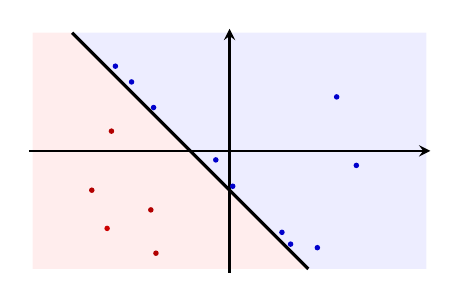
\begin{tikzpicture}[>=stealth, scale=0.5]
        \fill[blue!35!white, opacity = 0.2] (-4, 3) -- (5, 3) -- (5, -3) -- (2, -3)-- cycle;
        \fill[red!35!white, opacity = 0.2] (-4, 3) -- (-5, 3) -- (-5, -3) -- (2, -3)-- cycle;
        \draw[thick, ->] (-5.1, 0)-- (5.1, 0); 
        \draw[thick, ->] (0, -3.1) -- (0, 3.1); 
        \draw[very thick] (-4, 3) -- (2, -3); % node[above right]{\small $H = \{x + y + 1 = 0\}$}; 
        \fill[blue!80!black] (-2.9, 2.15) circle (2pt); 
        \fill[blue!80!black] (-2.49, 1.75) circle (2pt); 
        \fill[blue!80!black] (-1.93, 1.1) circle (2pt); 
        \fill[blue!80!black] (-0.35,-0.23) circle (2pt);
        \fill[blue!80!black] (0.08, -0.9) circle (2pt); 
        \fill[blue!80!black] (1.33, -2.07) circle (2pt);
        \fill[blue!80!black] (1.55, -2.37) circle (2pt); 
        \fill[blue!80!black] (2.23, -2.46) circle (2pt); 
        \fill[blue!80!black] (3.22, -0.37) circle (2pt); 
        \fill[blue!80!black] (2.72, 1.37) circle (2pt); 
        \fill[red!80!black] (-3.11, -1.97) circle (2pt);
        \fill[red!70!black] (-3, 0.5) circle (2pt); 
        \fill[red!70!black] (-3.5, -1) circle (2pt); 
        \fill[red!70!black] (-2, -1.5) circle (2pt); 
        \fill[red!70!black] (-1.87, -2.6) circle (2pt); 
    \end{tikzpicture}
    \caption{Many points near the decision boundary}
    \label{figure:close2decision}
\end{figure}

\end{frame}

%%%%
\begin{frame}
\frametitle{But\ldots data is messy}
If many points close to the decision boundary, likely for newly observed data to appear on ``wrong side'' of decision boundary. Perceptron algorithm gives us nothing to correct for this.

\pause
If ${\bf x}$ is close to decision boundary, we might feel less \emph{confident} in giving the label $h({\bf x})$ that we do. And, if ${\bf x}$ is farther from the boundary, where only one label is seen nearby, more confidence is warranted.

\pause
Also\ldots the immediate change of label across the boundary (a discontinuity in the model) \ldots perhaps not ``natural''?
\end{frame}

\section{Logistic model}

%%%%
\begin{frame}
\frametitle{Incorporating a probability into half-space model}
Instead of only capturing the sign of ${\bf w}\cdot{\bf x} + b$, compose it with the \textbf{logistic function}.    
    \[\sigma(z) = \frac{1}{1+e^{-z}}.\]
\begin{itemize}
    \item $0 < \sigma(z) < 1$ for all $z\in\mathbb R$;
    \item $\lim_{z\to\infty}\sigma(z) = 1$ and $\lim_{z\to-\infty}\sigma(z) = 0$;
    \item $\sigma(0) = 1/2$.
\end{itemize}

\centering
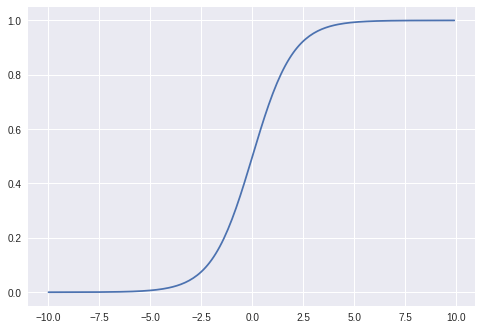
\includegraphics[height=0.3\textheight]{../../Images/logistic_function_graph.png}

\end{frame}

%%%%
\begin{frame}
\frametitle{Logistic model, continued}
    Define logistic model as follows.
    
    So, for ${\bf x}\in\mathbb R^d$, find $\sigma({\bf w}\cdot{\bf x}+b)$. 
    
    \pause
    Given ${\bf x}\in \mathbb R^d$, the side of the hyperplane $H$ it is on is determined by the sign of ${\bf w}\cdot{\bf x} + b$. Our half-space model: $h:\mathbb R^d\setminus H \to \{1,-1\}$.
    \pause
    \begin{itemize}
        \item (Positive side) Say that $h({\bf x}) = 1$ if ${\bf w}\cdot{\bf x}+b > 0$.
        \item (Negative side) Say that $h({\bf x}) = -1$ if ${\bf x}\cdot{\bf x}+b < 0$. 
    \end{itemize}

    \pause
    Given data with $\{\pm1\}$ labels, if there exists a hyperplane $H$ so that ${\bf x}$ has label $1$ if and only if it is on the positive side, the labeled data are called \textbf{linearly separable}. 

\end{frame}

%%%%
\begin{frame}
    \frametitle{Linearly separable}
    \begin{figure}[h!]
        \centering
        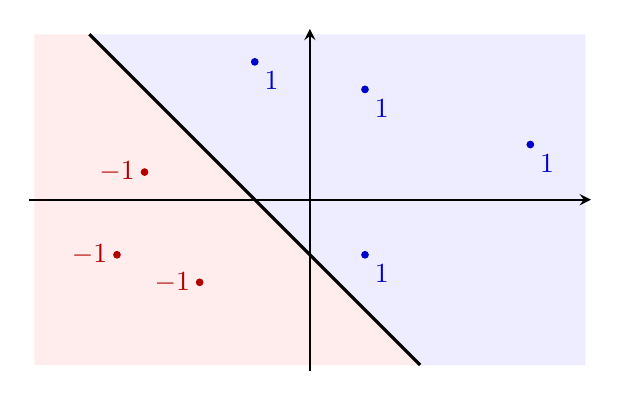
\begin{tikzpicture}[>=stealth, scale=0.7]
            \fill[blue!35!white, opacity = 0.2] (-4, 3) -- (5, 3) -- (5, -3) -- (2, -3)-- cycle;
            \fill[red!35!white, opacity = 0.2] (-4, 3) -- (-5, 3) -- (-5, -3) -- (2, -3)-- cycle;
            \draw[thick, ->] (-5.1, 0)-- (5.1, 0); 
            \draw[thick, ->] (0, -3.1) -- (0, 3.1); 
            \draw[very thick] (-4, 3) -- (2, -3); % node[above right]{\small $H = \{x + y + 1 = 0\}$}; 
            \fill[blue!80!black] (1, 2)node[below right]{$1$} circle (2pt); 
            \fill[blue!80!black] (-1, 2.5)node[below right]{$1$} circle (2pt); 
            \fill[blue!80!black] (1, -1)node[below right]{$1$} circle (2pt); 
            \fill[blue!80!black] (4, 1)node[below right]{$1$} circle (2pt); 
            \fill[red!70!black] (-3, 0.5)node[left]{$-1$} circle (2pt); 
            \fill[red!70!black] (-3.5, -1)node[left]{$-1$} circle (2pt); 
            \fill[red!70!black] (-2, -1.5)node[left]{$-1$} circle (2pt); 
        \end{tikzpicture}
        \caption{The hyperplane $H = \{(x_1,x_2)\in \mathbb R^2: x_1+ x_2+ 1 = 0\}$, corresponding positive and negative regions, ${\bf w} = (1, 1)$, $b = 1$}
        \label{figure:R2HyperplaneLabeled}
    \end{figure}
\end{frame}

%%%%
\begin{frame}
    \frametitle{Not linearly separable}
    \begin{figure}[h!]
        \centering
        \begin{tikzpicture}[>=stealth, scale=0.7]
            %\fill[blue!35!white, opacity = 0.2] (-4, 3) -- (5, 3) -- (5, -3) -- (2, -3)-- cycle;
            %\fill[red!35!white, opacity = 0.2] (-4, 3) -- (-5, 3) -- (-5, -3) -- (2, -3)-- cycle;
            \draw[thick, ->] (-5.1, 0)-- (5.1, 0); 
            \draw[thick, ->] (0, -3.1) -- (0, 3.1); 
            %\draw[very thick] (-4, 3) -- (2, -3); % node[above right]{\small $H = \{x + y + 1 = 0\}$}; 
            \fill[blue!80!black] (1, 2)node[below right]{$1$} circle (2pt); 
            \fill[red!70!black] (1, -1)node[below right]{$-1$} circle (2pt); 
            \fill[red!70!black] (-3, 0.5)node[left]{$-1$} circle (2pt); 
            \fill[blue!80!black] (-2, -1.5)node[left]{$1$} circle (2pt); 
        \end{tikzpicture}
        \caption{A data set in $\mathbb R^2$ that is not linearly separable.}
        \label{figure:notseparable}
    \end{figure}
    \pause
    \begin{itemize}
        \item A criterion (checkable, in theory) that is equivalent to ``not linearly separable''?
    \end{itemize}
\end{frame}

\section{Perceptron algorithm}

%%%%
\begin{frame}
    \frametitle{Setup for Perceptron algorithm}
    Labeled data: $({\bf x}_1, y_1), \ldots, ({\bf x}_n, y_n)$, with ${\bf x}_i\in\mathbb R^d$ and $y_i\in\{\pm1\}$ for all $i$.

    Assuming labeled data is linearly separable, the Perceptron algorithm is a procedure that is guaranteed to find a hyperplane that separates the data.\footnote{Introduced in \textit{The perceptron: A probabilistic model for information storage and organization in the brain}, F.~Rosenblatt, Psychological Review \textbf{65} (1958), 386{--}407.}
    
    \pause
    To describe it: for each ${\bf x}_i$, use $X_i$ to denote the $(d+1)$-vector consisting of ${\bf x}_i$ with $1$ appended at the end;

    Additionally, use $W$ to denote the vector ${\bf w}$ with $b$ appended at the end.

    \pause
    Note that $W\cdot X_i = {\bf w}\cdot{\bf x}_i + b$. 

    For linearly separable data, our goal is to find $W\in\mathbb R^{d+1}$ so that $W\cdot X_i$ and $y_i$ have the same sign (both positive or both negative), for all $1\le i\le n$.
    \begin{itemize}
        \item Equivalently, we need $y_i W\cdot X_i > 0$ for all $1\le i\le n$.
    \end{itemize}
\end{frame}

%%%%
\begin{frame}[fragile]
\frametitle{Perceptron algorithm}
Suppose the data is linearly separable. Also, \ttt{x} is an $n\times d$ array of points, with i$^{th}$ row equal to ${\bf x}_i$, and \ttt{y} is array of the labels. The Perceptron algorithm finds \ttt{W} iteratively as follows.\footnote{Recall, in pseudo-code block, left-facing arrow means \textit{assign} to variable on left.}
\pause 

\begin{pseudo}
input: x, y  ## x is n by d, y is 1d array
X = append 1 to each row of x
W = (0,0,...,0)  ## Initial W
while (exists i with y[i]*dot(W, X[i]) <= 0){
    W = W + y[i]*X[i]
}
return W
\end{pseudo}

\end{frame}

%%%%
\begin{frame}
    \frametitle{Example}
    A simple example in $\mathbb R^2$, with $n=4$ points.

    \begin{center}
    \ttt{x}: $\begin{bmatrix}-1 & 3 \\ -1 & -1 \\ 3 & -1 \\ 0 & 1.5\end{bmatrix}$  \qquad\qquad
    \ttt{y}: $\begin{bmatrix}-1 \\ -1 \\ 1 \\ 1\end{bmatrix}$
    \end{center}

    \centering
    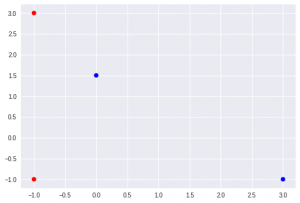
\includegraphics[height=0.3\textheight]{../../Images/ex2_data_halfspace.png}
\end{frame}

%%%%
\begin{frame}
    \frametitle{Example, continued}
    A simple example in $\mathbb R^2$, with $n=4$ points.

    \begin{center}
    \ttt{x}: $\begin{bmatrix}-1 & 3 \\ -1 & -1 \\ 3 & -1 \\ 0 & 1.5\end{bmatrix}$  \qquad\qquad
    \ttt{y}: $\begin{bmatrix}-1 \\ -1 \\ 1 \\ 1\end{bmatrix}$
    \end{center}

    Use $W^{(t)}$ for value of $W$ on step $t$. Start: $W^{(1)} = (0,0,0)$. \newline 
    Next step: $W^{(2)} = \vec{0} + y_1X_1 = -1\ast(-1,3,1) = (1,-3,-1)$.
    \pause
    
    Next: since $y_1W^{(2)}\cdot X_1 > 0$, check $y_2W^{(2)}\cdot X_2 = -1\ast(-1 + 3 -1) = -1$. \pause
    So, 
        \[W^{(3)} = W^{(2)} + y_2X_2 = (2, -2, -2).\]
    \pause 
    Continue in this way {--} on each step check dot products (in order) with $y_1X_1, y_2X_2, y_3X_3, y_4X_4$. Eventually you return the vector $W^{(10)} = (4, -0.5, 1)$. 
    
    \pause
    i.e., $H = \{(x_1,x_2)\in \mathbb R^2:\ 4x_1-0.5x_2 + 1 = 0\}$ separates the points.
\end{frame}

%%%%
\begin{frame}
    \frametitle{Perceptron algorithm, stopping time}
    Under our assumptions for Perceptron algorithm, a guarantee on eventually stopping.

    \begin{theorem}Define $R = \max_i|X_i|$ and $B = \min_i\{|V|: \forall i, y_iV\cdot X_i \ge 1\}$. Then, the Perceptron algorithm stops after at most $(RB)^2$ iterations and, when it stops with output $W$, then $y_iW\cdot X_i > 0$ for all $1\le i\le n$.
    \end{theorem}

    \pause 
    \textbf{Idea of proof:} Write $W^*$ for vector that realizes the minimum $B$. Also, write $W^{(t)}$ for the vector $W$ on the $t^{th}$ step, with $W^{(1)} = (0,0,\ldots,0)$.

    \pause
    Using how $W^{(t+1)}$ is obtained from $W^{(t)}$, can show that $W^*\cdot W^{(T+1)} \ge T$ after $T+1$ iterations. Also, using the condition on $W^{(T)}$ that necessitates an update, can show that $|W^{(T+1)}| \le \sqrt{T}R$. (Both statements, use induction.) 

    \pause
    Now, by Cauchy-Schwarz inequality, $T \le BR\sqrt{T}$, which we can rearrange to $T\le (BR)^2$.
\end{frame}

%%%%
\begin{frame}
    \frametitle{Another example, the Iris data set}
    First discussed by R.A.\ Fisher in a 1936 paper, Iris data set commonly used in explanations. It contains 150 points in $\mathbb R^4$, each for an individual iris flower from one of 3 species: Iris setosa, Iris virginica, and Iris versicolor.

    \onslide<2->{
    The 4 coordinates are measurements of sepal length, sepal width, petal length, and petal width (in cm).
    }

    \onslide<3->{
    Iris setosa points are linearly separable from the other two. \newline 
    Labels: \textit{Iris setosa} $\leftarrow$ 1; \textit{Other species} $\leftarrow$ -1.
    }

    \onslide<4->{
    Begin by opening the notebook \lstinline[language=Python,stringstyle=\ttfamily\color{strings}]{'perceptron-iris-notebook.ipynb'} \ldots 
    After completing the algorithm, should get final $W = ({\bf w}, b)$, where ${\bf w} = (1.3,4.1,-5.2,-2.2)$ and $b = 1$.
    }

    \onslide<1->{
    \begin{figure}
    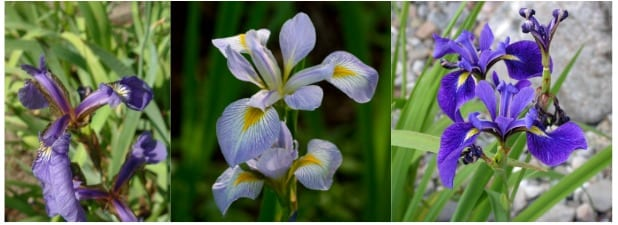
\includegraphics[height=0.2\textheight]{../../Images/iris-3species.jpg}
    \caption{Images by G.\ Robertson, E.\ Hunt, Radomil \copyright CC BY-SA 3.0}
    \end{figure}
    }
\end{frame}
\end{document}